

\tikzset{every picture/.style={line width=0.75pt}} %set default line width to 0.75pt        

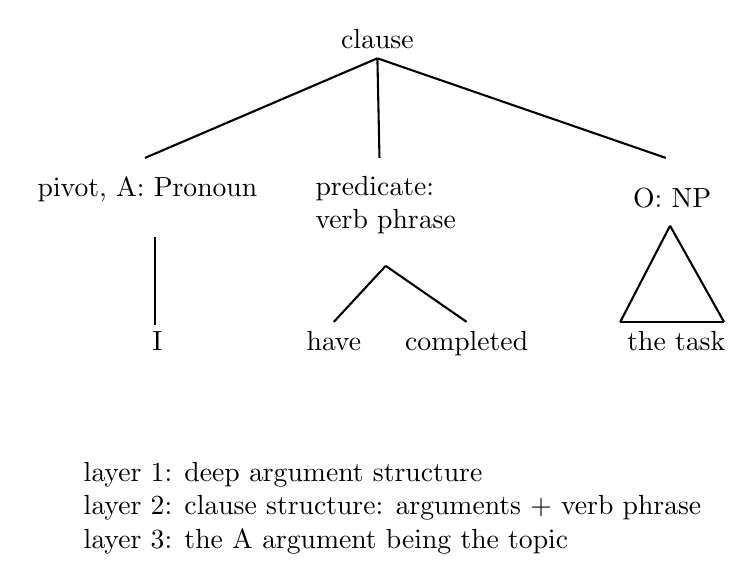
\begin{tikzpicture}[x=0.75pt,y=0.75pt,yscale=-1,xscale=1]
%uncomment if require: \path (0,390); %set diagram left start at 0, and has height of 390

%Straight Lines [id:da4161051988460063] 
\draw    (183,100.81) -- (71,148.81) ;
%Straight Lines [id:da36248311433047187] 
\draw    (187,200.81) -- (162,227.81) ;
%Straight Lines [id:da4439661314753782] 
\draw    (187,200.81) -- (226,227.81) ;
%Straight Lines [id:da36890954567869483] 
\draw    (300,227.81) -- (350,227.81) ;
%Straight Lines [id:da011342458373226894] 
\draw    (324,181.48) -- (300,227.81) ;
%Straight Lines [id:da5435200709744346] 
\draw    (324,181.48) -- (350,227.81) ;
%Straight Lines [id:da24568188379824396] 
\draw    (76,186.81) -- (76,229.48) ;
%Straight Lines [id:da3308532295080375] 
\draw    (183,100.81) -- (184,148.81) ;
%Straight Lines [id:da7487945318074942] 
\draw    (183,100.81) -- (322,148.81) ;

% Text Node
\draw (77,230.81) node [anchor=north] [inner sep=0.75pt]   [align=left] {I};
% Text Node
\draw (162,230.81) node [anchor=north] [inner sep=0.75pt]   [align=left] {have};
% Text Node
\draw (226,230.81) node [anchor=north] [inner sep=0.75pt]   [align=left] {completed};
% Text Node
\draw (327,230.81) node [anchor=north] [inner sep=0.75pt]   [align=left] {the task};
% Text Node
\draw (187,187) node [anchor=south] [inner sep=0.75pt]   [align=left] {predicate:\\verb phrase};
% Text Node
\draw (325,174) node [anchor=south] [inner sep=0.75pt]   [align=left] {O: NP};
% Text Node
\draw (15,157) node [anchor=north west][inner sep=0.75pt]   [align=left] {\begin{minipage}[lt]{83.56pt}\setlength\topsep{0pt}
\begin{center}
pivot, A: Pronoun
\end{center}

\end{minipage}};
% Text Node
\draw (183,97.81) node [anchor=south] [inner sep=0.75pt]   [align=left] {clause};
% Text Node
\draw (40,294) node [anchor=north west][inner sep=0.75pt]   [align=left] {layer 1: deep argument structure\\layer 2: clause structure: arguments + verb phrase\\layer 3: the A argument being the topic};


\end{tikzpicture}
